%%%%%%%%%%%%%%%%%%%%%%%%%%%%%%%%%%%%%%%%%
% Article EcoFoG
% Version 2.1 (23/10/2017)
%
% adapté de :
% Stylish Article
% LaTeX Template
% Version 1.0 (31/1/13)
%
% This template has been downloaded from:
% http://www.LaTeXTemplates.com
%
% Original author:
% Mathias Legrand (legrand.mathias@gmail.com)
%
% License:
% CC BY-NC-SA 3.0 (http://creativecommons.org/licenses/by-nc-sa/3.0/)
%
%%%%%%%%%%%%%%%%%%%%%%%%%%%%%%%%%%%%%%%%%


%----------------------------------------------------------------------------------------
%	PACKAGES AND OTHER DOCUMENT CONFIGURATIONS
%----------------------------------------------------------------------------------------

\documentclass[fleqn,10pt]{ArtEcoFoG} % Document font size and equations flushed left

\setcounter{tocdepth}{3} % Show only three levels in the table of contents section: sections, subsections and subsubsections


% Pandoc environments
\usepackage{framed}
\usepackage{fancyvrb}
\providecommand{\tightlist}{%
  \setlength{\itemsep}{0pt}\setlength{\parskip}{0pt}}
\newcommand{\VerbBar}{|}
\newcommand{\VERB}{\Verb[commandchars=\\\{\}]}
\DefineVerbatimEnvironment{Highlighting}{Verbatim}{commandchars=\\\{\}, fontsize=\scriptsize} % Code R
\definecolor{shadecolor}{RGB}{248,248,248}
\newenvironment{Shaded}{\begin{snugshade}}{\end{snugshade}}
\newcommand{\KeywordTok}[1]{\textcolor[rgb]{0.13,0.29,0.53}{\textbf{{#1}}}}
\newcommand{\DataTypeTok}[1]{\textcolor[rgb]{0.13,0.29,0.53}{{#1}}}
\newcommand{\DecValTok}[1]{\textcolor[rgb]{0.00,0.00,0.81}{{#1}}}
\newcommand{\BaseNTok}[1]{\textcolor[rgb]{0.00,0.00,0.81}{{#1}}}
\newcommand{\FloatTok}[1]{\textcolor[rgb]{0.00,0.00,0.81}{{#1}}}
\newcommand{\ConstantTok}[1]{\textcolor[rgb]{0.00,0.00,0.00}{{#1}}}
\newcommand{\CharTok}[1]{\textcolor[rgb]{0.31,0.60,0.02}{{#1}}}
\newcommand{\SpecialCharTok}[1]{\textcolor[rgb]{0.00,0.00,0.00}{{#1}}}
\newcommand{\StringTok}[1]{\textcolor[rgb]{0.31,0.60,0.02}{{#1}}}
\newcommand{\VerbatimStringTok}[1]{\textcolor[rgb]{0.31,0.60,0.02}{{#1}}}
\newcommand{\SpecialStringTok}[1]{\textcolor[rgb]{0.31,0.60,0.02}{{#1}}}
\newcommand{\ImportTok}[1]{{#1}}
\newcommand{\CommentTok}[1]{\textcolor[rgb]{0.56,0.35,0.01}{\textit{{#1}}}}
\newcommand{\DocumentationTok}[1]{\textcolor[rgb]{0.56,0.35,0.01}{\textbf{\textit{{#1}}}}}
\newcommand{\AnnotationTok}[1]{\textcolor[rgb]{0.56,0.35,0.01}{\textbf{\textit{{#1}}}}}
\newcommand{\CommentVarTok}[1]{\textcolor[rgb]{0.56,0.35,0.01}{\textbf{\textit{{#1}}}}}
\newcommand{\OtherTok}[1]{\textcolor[rgb]{0.56,0.35,0.01}{{#1}}}
\newcommand{\FunctionTok}[1]{\textcolor[rgb]{0.00,0.00,0.00}{{#1}}}
\newcommand{\VariableTok}[1]{\textcolor[rgb]{0.00,0.00,0.00}{{#1}}}
\newcommand{\ControlFlowTok}[1]{\textcolor[rgb]{0.13,0.29,0.53}{\textbf{{#1}}}}
\newcommand{\OperatorTok}[1]{\textcolor[rgb]{0.81,0.36,0.00}{\textbf{{#1}}}}
\newcommand{\BuiltInTok}[1]{{#1}}
\newcommand{\ExtensionTok}[1]{{#1}}
\newcommand{\PreprocessorTok}[1]{\textcolor[rgb]{0.56,0.35,0.01}{\textit{{#1}}}}
\newcommand{\AttributeTok}[1]{\textcolor[rgb]{0.77,0.63,0.00}{{#1}}}
\newcommand{\RegionMarkerTok}[1]{{#1}}
\newcommand{\InformationTok}[1]{\textcolor[rgb]{0.56,0.35,0.01}{\textbf{\textit{{#1}}}}}
\newcommand{\WarningTok}[1]{\textcolor[rgb]{0.56,0.35,0.01}{\textbf{\textit{{#1}}}}}
\newcommand{\AlertTok}[1]{\textcolor[rgb]{0.94,0.16,0.16}{{#1}}}
\newcommand{\ErrorTok}[1]{\textcolor[rgb]{0.64,0.00,0.00}{\textbf{{#1}}}}
\newcommand{\NormalTok}[1]{{#1}}
\usepackage{longtable,booktabs}
\usepackage{caption}
% These lines are needed to make table captions work with longtable:
\makeatletter
\def\fnum@table{\tablename~\thetable}
\makeatother
% longtable 2 columns
% https://tex.stackexchange.com/questions/161431/how-to-solve-longtable-is-not-in-1-column-mode-error
\makeatletter
\let\oldlt\longtable
\let\endoldlt\endlongtable
\def\longtable{\@ifnextchar[\longtable@i \longtable@ii}
\def\longtable@i[#1]{\begin{figure}[t]
\onecolumn
\begin{minipage}{0.5\textwidth}\scriptsize
\oldlt[#1]
}
\def\longtable@ii{\begin{figure}[t]
\onecolumn
\begin{minipage}{0.5\textwidth}\scriptsize
\oldlt
}
\def\endlongtable{\endoldlt
\end{minipage}
\twocolumn
\end{figure}}
\makeatother

\usepackage{graphicx,grffile}
\makeatletter
\def\maxwidth{\ifdim\Gin@nat@width>\linewidth\linewidth\else\Gin@nat@width\fi}
\def\maxheight{\ifdim\Gin@nat@height>\textheight0.8\textheight\else\Gin@nat@height\fi}
\makeatother
% Scale images if necessary, so that they will not overflow the page
% margins by default, and it is still possible to overwrite the defaults
% using explicit options in \includegraphics[width, height, ...]{}
\setkeys{Gin}{width=\maxwidth,height=\maxheight,keepaspectratio}

% User-adder preamble
\usepackage{textcomp} \DeclareUnicodeCharacter{B0}{\textdegree}
\usepackage{tabu}
\renewenvironment{table}{\begin{table*}}{\end{table*}\ignorespacesafterend}
\hyphenation{bio-di-ver-si-ty sap-lings}

%----------------------------------------------------------------------------------------
%	ARTICLE INFORMATION
%----------------------------------------------------------------------------------------

\JournalInfo{Hal 00679993} % Journal information
\Archive{DOI xxxx} % Additional notes (e.g. copyright, DOI, review/research article)

\PaperTitle{30 Years of Post-disturbance Recruitment in Tropical Forest} % Article title

\Authors{
Ariane MIRABEL\textsuperscript{1*}\\ Eric MARCON\textsuperscript{1}\\ Bruno HERAULT\textsuperscript{2}
} % Authors
\affiliation{
\textsuperscript{1}UMR EcoFoG, AgroParistech, CNRS, Cirad, INRA, Université des Antilles,
Université de Guyane.\\ \hspace{1em} Campus Agronomique, 97310 Kourou, France.\\\textsuperscript{2}INPHB (Institut National Ploytechnique Félix Houphoüet Boigny)\\ \hspace{1em} Yamoussoukro, Ivory Coast
}
\affiliation{*\textbf{Corresponding author}: ariane.mirabel@ecofog.gf, http://www.ecofog.gf/spip.php?article47} % Corresponding author

\Keywords{Taxonomic and Functional Diversity, Recruitment, Resilience, Tropical Forests, Disturbance Dynamics} % Keywords - if you don't want any simply remove all the text between the curly brackets
\newcommand{\keywordname}{Keywords} % Defines the keywords heading name

%----------------------------------------------------------------------------------------
%	ABSTRACT
%----------------------------------------------------------------------------------------

\Abstract{
Résumé de l'article.
}

%----------------------------------------------------------------------------------------

\begin{document}

\selectlanguage{english}

\flushbottom % Makes all text pages the same height

\maketitle % Print the title and abstract box

\tableofcontents % Print the contents section

\thispagestyle{empty} % Removes page numbering from the first page

%----------------------------------------------------------------------------------------
%	ARTICLE CONTENTS
%----------------------------------------------------------------------------------------


\section{Introduction}\label{introduction}

Determining the response of tropical forests to disturbance is a key to
predict their fate in the global changing context. In the last decades,
tropical forests experienced a wide range of disturbance, from radical
land-use changes for agriculture or mining
\citep{Dezecache2017a, Dezecache2017b} to more insidious changes of
communities structure, diversity and functioning following anthropogenic
activities like selective logging \citep{Baraloto2012a, Herault2016} or
climate change \citep{Aubry-Kientz2015}. In that respect a vast
literature successfully modeled communities response to disturbance in
terms of tree growth \citep{Gourlet-Fleury2000}, tree height
\citep{Rutishauser2016}, carbon stocks and fluxes
\citep{Putz2012, Martin2015, Piponiot2016}. Similar approaches regarding
forest composition and diversity, however, have been hindered by the
huge biological diversity, often focusing on common or mainly commercial
species, and the scarcity of long-term monitoring
\citep{Sebbenn2008, Rozendaal2010, Vinson2015}.

Communites trajectories after disturbance, defined here as the evolution
of communities diversity along time, depend on the trees surviving from
before disturbance and on those recruited afterward \citep{Herault2018}.
Because surviving trees proved to mirror the composition of
pre-disturbance forest, the response of communities is driven by the
diversity and composition of recruited trees that build the future
community and determine the resilience of the pre-disturbance forest.
The recruitment trajectories are first determined by the composition and
diversity of the initial community that partly conditions the pool of
recruitable species \citep{Herault2018}. Trajectories then depend on the
recruitment processes that are either stochastic, like random dispersal,
recruitment and death \citep{Hubbell2001}, or deterministic, like
niche-based competition processes \citep{Adler2007} While stochastic
processes build communities as random samples of the larger
regional-scale forest, deterministic processes rely on the abiotic
environment and filter-out recruited species according to their ecology.
To understand the mechanisms of communities trajectories the first point
is to estimate the importance of the initial community composition and
the balance between stochastic and deterministic processes. Then it is
to determine the resilience of communities and the time to recover
pre-disturbance ecosystem properties in order to adjust exploitation and
conservation guidelines \citep{Diaz2005, Gardner2007, Schwartz2017}.

The ecological processes shaping communities' trajectories differently
affect their functional and taxonomic diversities as the first consider
all species equally while the second accounts for species functioning
and ecology \citep{Violle2007b, Kunstler2016}. The potential decoupling
between functional and taxonomic trajectories is then insightful of the
ecological processes at stake, and only a combined approach of
functional and taxonomic diversities would reveal the determinant
recruitment processes \citep{Fukami2005}. Functional trajectories will
rely on deterministic processes oriented towards the use of limiting
resources: in tropical forests where the light is limiting forests
response would then be a shift from slow-growing, long-living species
with ``conservative'' resource use to fast growing, resource
``acquisitive'' species \citep{Denslow1980, Molino2001, Bongers2009}.\\
Such processes would be detected throught the diversity and composition
trajectories of key leaf, wood and life-history functional traits
assessing species ecology and resources acquisition strategy
\citep{Wright2004, Chave2009b, Herault2011}. The deterministic processes
could filtered-out, decreasing the recruitment functional diversity, or
the less competitive ones could be excluded, increasing the functional
diversity through the limitation of similarity among species
\citep{Ackerly2003, McGill2006}.

In this paper we followed the fate of a recruited tree communities
(60121 individuals) over 30 years on a large disturbance gradient, with
10 to 60\% of forest biomass removed. We assessed the taxonomic and
functional diversity of recruited trees and the corresponding traits
trajectories, using a large functional trait database covering the leaf,
wood and life-history spectra. We besides followed along time the
composition dissimilarity of recruited trees compared to the initial
communities. Eventually we compared the observed trajectories to a
stochastic recruitment entailing the random sampling of recruits and the
randomization of their functional traits. These trajectories aimed (i)
to assess the role of deterministic processes compared to stochastic
recruitment after disturbance, (ii) assess the taxonomic and functional
convergence of forest communities and the maintenance of taxonomic
composition in the long term, and (iii) determine the degree of
resilience of the ecosystem.

\section{Material and Methods}\label{material-and-methods}

\subsection{Study Site}\label{study-site}

The Paracou station is located in a lowland tropical rain forest in
French Guiana (5°18'N and 52°53'W). Climate is tropical wet with mean
annual precipitation averaging 2980 mm.y\textsuperscript{-1} (30-y
period) and a 3-months dry season (\textless{} 100
mm.months\textsuperscript{-1}) from mid-August to mid-November, and a
one-month dry season in March \citep{Wagner2011}. Elevation ranges from
5 to 50 m and mean annual temperature is 26°C. Soils are thin acrisols
over a layer of transformed saprolite with low permeability generating
lateral drainage during heavy rains. The disturbance experiment spread
over a network of twelve 6.25ha plots (Table \ref{tab:Tab1}) that
underwent three disturbance treatments in 1986-1987 \citep{Herault2018}.
Dominant families are Fabaceae, Chrysobalanaceae, Lecythidaceae and
Sapotaceae.

\begin{table}

\caption{\label{tab:Tab1}Intervention table, summary of the disturbance intensity for the 4 plot treatments in Paracou.}
\centering
\begin{tabu} to \linewidth {>{\raggedright}X>{\raggedright}X>{\raggedright}X>{\raggedright}X>{\raggedright}X}
\toprule
Treatment & Timber & Thinning & Fuelwood & \%AGB lost\\
\midrule
Control &  &  &  & 0\\
T1 & DBH $\geq$ 50 cm, commercial species, $\approx$ 10 trees/ha &  &  & $[12\%-33\%]$\\
T2 & DBH $\geq$ 50 cm, commercial species, $\approx$ 10 trees/ha & DBH $\geq$ 40 cm, non-valuable species, $\approx$ 30 trees/ha &  & $[33\%-56\%]$\\
T3 & DBH $\geq$ 50 cm, commercial species, $\approx$ 10 trees/ha & DBH $\geq$ 50 cm, non-valuable species, $\approx$ 15 trees/ha & 40 cm $\leq$ DBH $\leq$ 50 cm, non-valuable species, $\approx$ 15 trees/ha & $[35\%-56\%]$\\
\bottomrule
\end{tabu}
\end{table}

\subsection{Inventories Protocol and Dataset
Collection}\label{inventories-protocol-and-dataset-collection}

All trees above 10 cm DBH were mapped and measured annually since 1984.
During inventories, trees were first identified with a vernacular name
assigned by the field team, and afterward with a scientific name
assigned by a botanist during regular botanical campaigns. Botanical
campaigns have been carried out every 5 to 6 years from 2003 onwards.
These changes in identification protocol raised methodological issues as
vernacular names usually correspond to different botanical species,
resulting in significant taxonomic uncertainties that were propagated to
composition and diversity metrics. Vernacular names were replaced
through multinomial trials
\(M_v\Big(\big[s_1, s_2, …, s_N\big],\big[\alpha_1, \alpha_2,…, \alpha_3\big]\Big)\)
based on the observed association probability
\(\big[\alpha_1, \alpha_2,…, \alpha_3\big]\) between each vernacular
name \emph{v} and the species \(\big[s_1, s_2, …, s_N\big]\) recorded in
the inventory. See appendix 1 and \citet{Aubry-Kientz2013} for the
detailed methodology. To avoid remaining identification caveats, the
simulated botanical inventories were reported at genus level.

Eight functional traits were considered, representing leaf economics
(leaves thickness, toughness, total chlorophyll content and specific
leaf area), wood economics (wood specific gravity and bark thickness)
and life history traits (maximum specific height and seed mass). Traits
were exctracted from the BRIDGE project \footnote{http://www.ecofog.gf/Bridge/}
where trait values were measured on nine forest plots infrench guianan,
including two in Paracou. Missing trait values of the trait database
(10\%) were filled by multivariate imputation by chained equation using
the Mice r package \citep{Mice2011}. As traits variability was lower
within genus and families, we accounted for the phylogenetic signal of
the functional traits by restricting the gap filling processes to
samples pertaining to the next higher taxonomic level. As seed mass
information corresponded to a classification into discrete mass classes,
no data filling process was applied so analysis were performed only
considering the 414 botanical species of the seed mass dataset.

\subsection{Recruitment trajectories}\label{recruitment-trajectories}

To disentangle the recruitment processes from overall dynamics,
communities were split into per-disturbance surviving trees and those
recruited since disturbance. Recruited communities were examined either
considering the ``punctual recruitment'', \emph{i.e.} recruited trees by
2-year intervals, or all recruits since disturbance as the ``accumulated
recruits''. Eventually, in disturbed plots the recruited communities
were examined distinguishing the undisturbed and logging gap areas to
test the validity of recruitment processes for the whole area.

The taxonomic diversity was assessed through Richness and the Hill
number translation of Shannon and Simpson indices
\citep{Hill1973, chao2015estimating, Marcon2015b}.\\
The three diversities belong to the set of HCDT or generalized entropy,
respectively corresponding to the 0, 1 and 2 order of diversity
(\emph{q}), which grasps the balance between richness and evenness in
the community through the value of \emph{q} that emphasizes common
species. Functional trajectories were estimated with the Rao quadratic
entropy and completed by the trajectories of traits community weighted
means (CWM), representing the average trait value in a community
weighted by relative abundance of the species carrying each value
\citep{Diaz2007, Garnier2004}. Seed mass trajectories were reported by
the proportion of each class recorded in the inventories. The similarity
between the recruited trees and the pre-disturbance forest was measured
with the turnover metrics detailed in \citet{Podani2013a}. To estimate
the importance of stochastic processes the recruitment was compared to
the trajectories of a random sampling. For the taxonomic trajectories
the random sampling was a shuffle of trees among plots that preserved
species abundance and tree density, and for the functional diversity it
was a shuffling of functional trait values among species.

All composition and diversity metrics correspond to the median and 90\%
percentile obtained after 50 iterations of the taxonomy uncertainty
propagation framework and the gap filling process. The stochastic
trajectories were similarily obtained after 50 iterations of the random
sampling.

\section{Results}\label{results}

\subsection{Recruitment Diversity}\label{recruitment-diversity}

All the trajectories were identical in disturbed and undisturbed areas,
confirming that the recruitment processes applied to whole communities
and were not restricted to logging gaps.

\subsubsection{Taxonomic Diversity}\label{taxonomic-diversity}

The diversity trajecctories of punctual recruitment followed a
consistent trajectory after disturbance with first an increase of the
richness and a decrease of the evenness (Figure (\ref{fig:DivTraj}). For
all disturbed plots,both richness and evenness tended to return towards
initial values but none had recovered 30 years after disturbance. The
accumulated recruits displayed sharp increasing richness (order 0) and
decreasing evenness (order 2) after intense disturbance (T3 and some T2,
Appendix I, fig. S1).

\begin{figure*}

{\centering 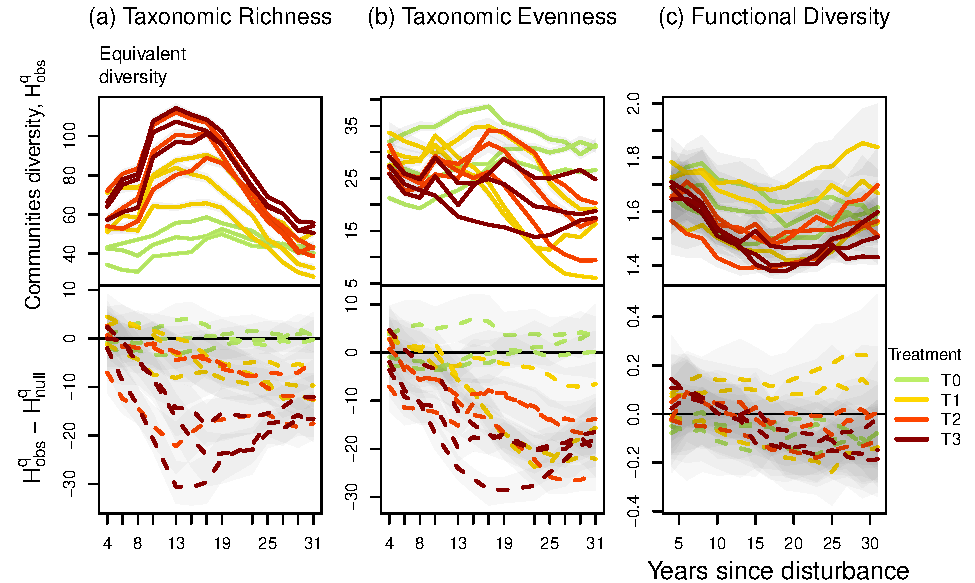
\includegraphics[width=0.8\linewidth]{RecruitmentTrajectories_files/figure-latex/DivTraj-1} 

}

\caption{Trajectories of Richness, Shannon and Simpson diversity for 2-years laps punctual  recruitment (upper panels) and divergence to null model (lower panels). Lines colors refer to the perturbation regime: green for control, blue for T1, orange for T2 and red for T3 disturbance treatments. Plain lines correspond to the median observed after uncertainty propagation and are given along with the 95\% confidence interval (grey envelope).}\label{fig:DivTraj}
\end{figure*}

Punctual and accumulated recruitment diversities were then compared to
the stochastic trajectories of a random sampling. Richness (order 0) and
evenness (order 2) of punctual recruits remained equivalent or higher
than for a random sampling in control plots while both were lower in
disturbed plots. Disturbed plots however followed humped-shaped
trajectories heading towards a recovery of the initial state (Figure
\ref{fig:DivTraj}). Accumulated recruitment richness and evenness were
higher or equivalent to those of the random sampling after low
disturbance intensity (plots T1 and some plots T2) but lower after
intense disturbance (plots T3 and a plot T2, Appendix I fig. S1).

\subsubsection{Functional Diversity and
Composition}\label{functional-diversity-and-composition}

Communities functional diversity was measured with the Rao diversity and
compared to the stochastic trajectories of a random traits shuffling. In
disturbed plots (T2 and T3), the functional diversity decreased until 15
years after disturbance (Figure \ref{fig:FunTraj}) before recovering
towards the initial values. While the recovery was not achieved for the
most disturbed plots, the functional diversity of lighter disturbance
plots recovered faster and for some T1 plots exceeded the initial
values. For all plots, disturbed or not, the observed functional
diversity was lower than this of the random model, to the exception of
two plots T1.

\begin{figure}

{\centering 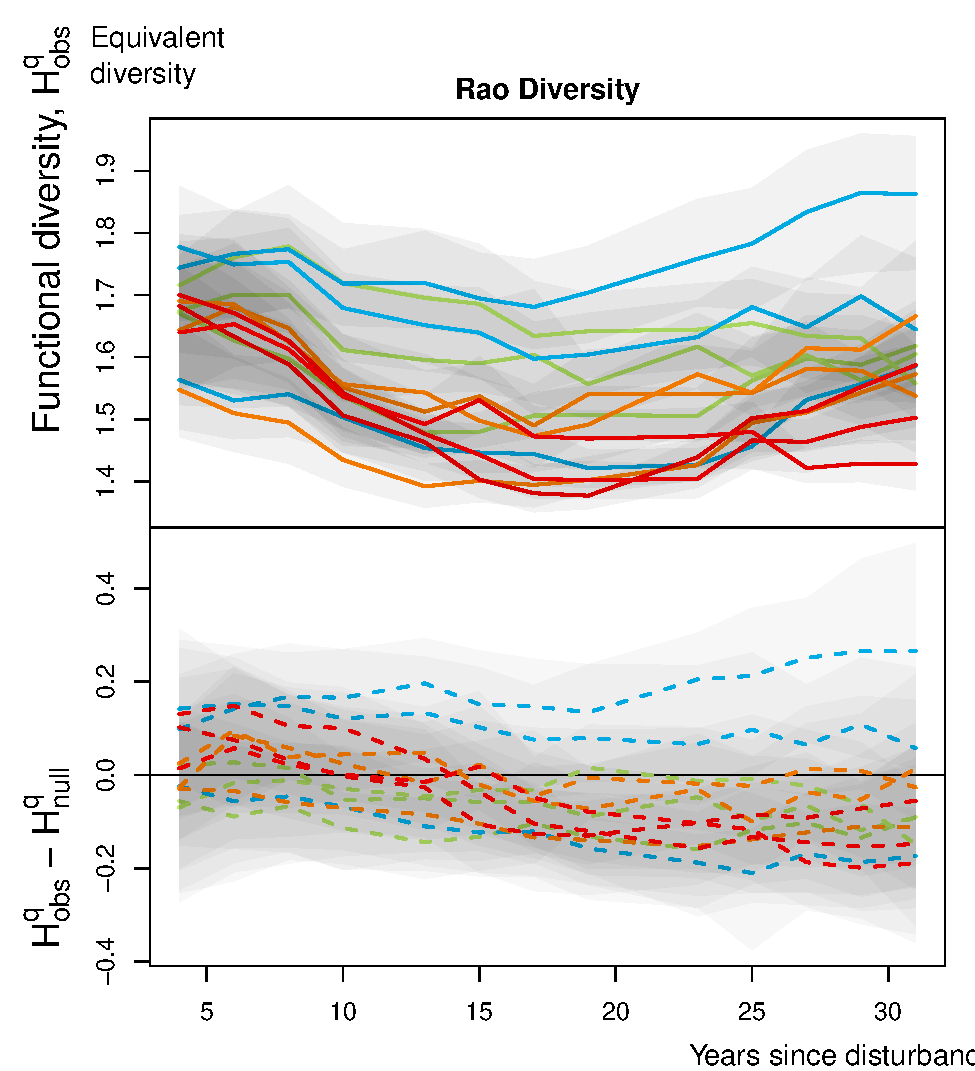
\includegraphics{RecruitmentTrajectories_files/figure-latex/FunTraj-1} 

}

\caption{Functional diversity of punctual recruited trees from the considered functional traits and divergence to null model. Values reported correspond to the plot-level median and the 95\% confidence interval obtained after 50 repetition of the taxonomic uncertainty propagation and the functional database gap-filling processes and 50 run of the null model. Lines colors correspond to the logging treatment initially applied (green for control, blue for T1,orange for T2 and red for T3).}\label{fig:FunTraj}
\end{figure}

Trajectories of the functional traits showed a switch in disturbed plots
towards species with large exchange surface area, light tissues (high
SLA, low leaf toughness and thickness and low wood specific gravity)
with smaller maximum height (Figure \ref{fig:CWM}). Functional traits
either followed hump-shaped trajectories with an ongoing recovery or an
achieved return to the initial state (for SLA,Bark thickness and leaf
thickness and Hmax to a certain extent).

\begin{figure*}

{\centering 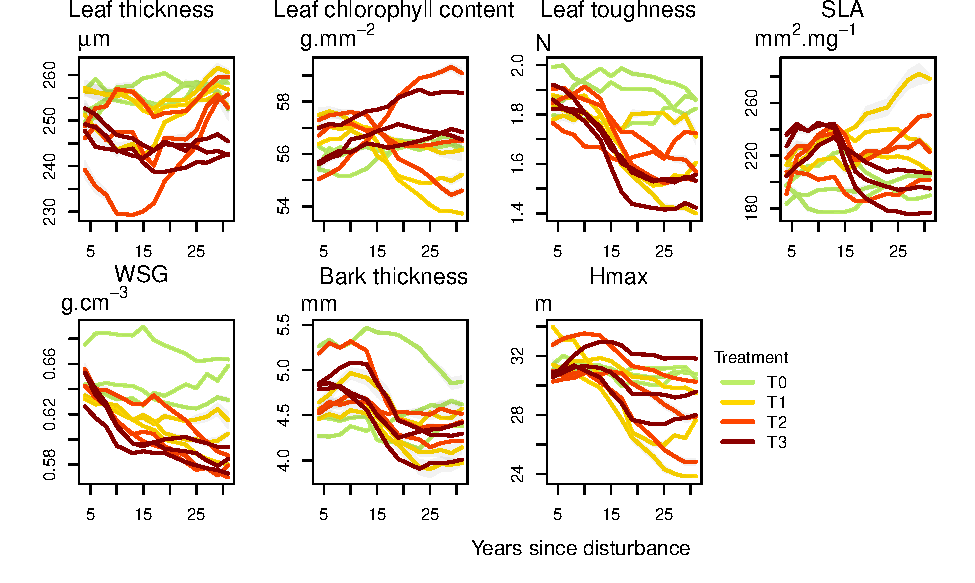
\includegraphics[width=0.8\linewidth]{RecruitmentTrajectories_files/figure-latex/CWM-1} 

}

\caption{Community weighted means (CWM) of the four disturbance treatment for the four leaf traits, the two stem traits  and the specific Hmax. Values reported correspond to the plot-level median obtained after 50 repetition of the taxonomic uncertainty propagation and the functional database gap-filling processes. Lines colors correspond to the disturbance intensity (green for control, blue for T1,orange for T2 and red for T3).}\label{fig:CWM}
\end{figure*}

\subsection{Recruitment Turnover}\label{recruitment-turnover}

In control plots species turnover remained highly stable for the 30
sampled years (Figure \ref{fig:Turnover}), reflecting a strong
similarity between the initial plots composition and the punctual
recruits. In disturbed plots, the taxonomic turnover followed a marked
hump-backed trajectory, with a maximum value reached around 15 years
after disturbance and a maximum positively correlated to the disturbance
intensity (\(\rho_{spearman}=0.93\)). Thirty years after disturbance the
turnover of all disturbed plots had return to low values close to zero.

\begin{figure}

{\centering 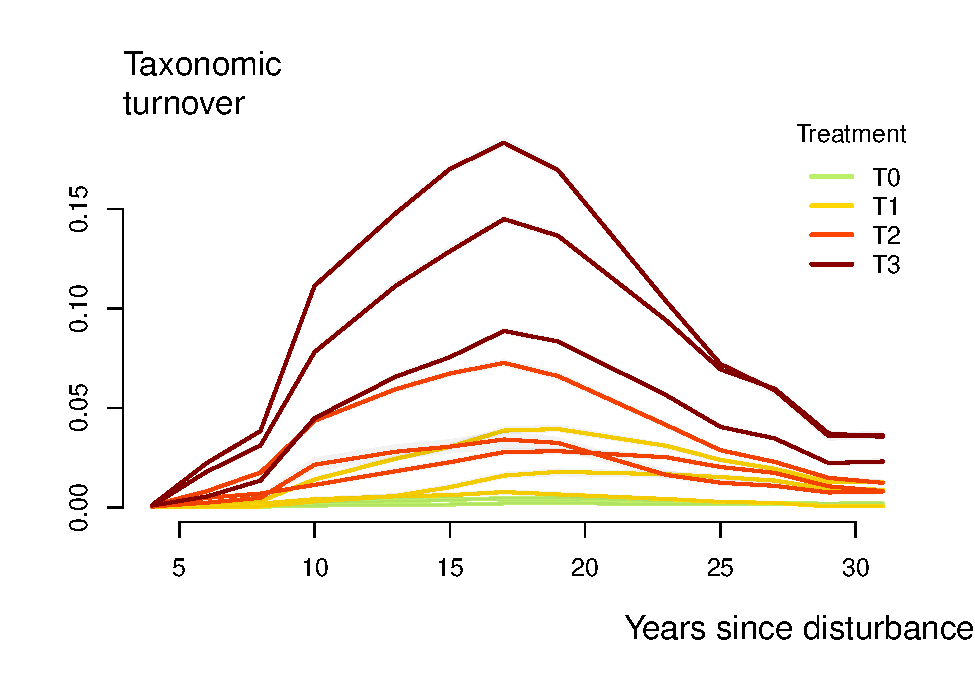
\includegraphics{RecruitmentTrajectories_files/figure-latex/Turnover-1} 

}

\caption{Trajectories over the 30 sampled years of the abundance-based turnover between recruited trees and intial communities before disturbance. Grey envelopes correspond to the 0.025 and 0.975 percentiles of the uncertainty propagation procedue and lines to the median in green for control, blue for T1,orange for T2 and red for T3).}\label{fig:Turnover}
\end{figure}

\section{Discussion}\label{discussion}

\subsection{The three recruitment phases of communities
trajectories}\label{the-three-recruitment-phases-of-communities-trajectories}

Along the 30 years, the recruitment richness and species turnover
compared to the initial composition, and the trajectories of key
functional traits (SLA and bark thickness) exhibited clear hump-shaped
trajectories, revealing three distinct recruitment phases. Communities
trajectories involved an interplay between stochastic and deterministic
recruitment, advocating that disturbance effectively maintained forests
diversity \citep{Molino2001, Sheil2003}.

As a first step (0-8 years), recruited trees showed low turnover
compared to the initial composition and matched the functoinal diversity
of a stochastic recruitment process. This first recruitment phase
mirroring the old-growth pre-disturbance community then likely involved
already grown saplings (DBH \textless{}10cm) immediatly benefitting from
the increased enlightment and the alleviated competition induced by
disturbance \citep{Herault2010}.

A second phase (8-15 years) then fall into place, corresponding to
marked changes in several functional traits trajectories and to a
decrease in the evenness and functional diversity of the recruited
species. These changes revealed during the second phase a restriction in
the pool of recruited species, likely selected based on their functional
strategy. Indeed after intense disturbance, sharp changes in the SLA,
wood density and leaf thickness trajectories revealed the prominent
recruitment of short-lived, fast growing hard pionneers species with
competitive and efficient light acquisition
\citep{Wright2004, Chave2009b, Herault2011, Reich2014}.\\
The second phase likely incorporated true recruits, \emph{i.e.} trees
germinated from the seed bank, selected according to their resource
acquisition strategy. The stochastic recruitment observed in the first
place were therefore balanced with deterministic, niche-based
competition processes. Along time diversity trajectories returned
towards the initial state and the values of stochastic recruitment,
revealing a reversed balance where stochastic recruitment progressively
prevailing again. The balance along time between deterministic and
stochastic processes was determined by the initial disturbance
intensity. After light disturbance (T1 plots), although the pool of
recruited species was restricted by the competitive exclusion for
resources the turnover compared to initial state remained low. Recruited
trees then still mirrored the pre-disturbance communities but recruited
species were more pioneers and light demanders, with strategies of
efficient resource acquisition (high SLA and leaf chlorophyll content)
and inexpensive, short-lived tissues (low leaf thickness and thoughness,
small Hmax and low wood density and bark thickness)
\citep{Hubbell1999, Sheil2003, Bongers2009}. At this disturbance
intensity the recruitment evenness and functional diversity remained
high so despite the selection of more light-demanding species the
recruitment was not overwhelmed by hard pioneers. This might be
explained by the recruitment and dispersal limitations due to the short
dispersal distance observed for tropical trees, specifically in Paracou
with the genetic clumping of some pioneers
\citep{Leclerc2015, Scotti2015a}. After intense disturbance in contrast
(T2 and T3 plots), the recruitment rapidly differed from the
pre-disturbance composition and corresponded to a sharp increase of the
SLA and bark thickness. These drastic trajectories changes reflected an
overhelming recruitment of hard pioneers likely entailing significant
changes in communities functioning \citep{Diaz2005}.

A third recruitment phase eventually entailed a progressive recovery of
the functional diversity revealing more diversified recruitment.
Recruited species remained mainly light-demanding and therefore still
underwent deterministic competition processes, but their composition
increasingly mirrored the pre-disturbance community which revealed a
progressive recovery of stochastic recruitment processes.

\subsection{The questioned completeness of communities
resilience}\label{the-questioned-completeness-of-communities-resilience}

After 30 years, although taxonomic and functional diversity had
recovered initial values, the recruitment processes remained submitted
to the deterministic selection of recruited species in contrast with the
stochastic recruitment of undisturbed forests. The recruitment processes
proved then consistently resilient but after long time period.

The recovery of recruitment processes meant the convergence of
communities towards their initial, pre-disturbance state. More than
commonly thought, the taxonomic trajectory of ecosystems relied on their
pre-disturbance characteristics and concur to maintain the initial
taxonomic differences among local communities \citep{Anderson2007}. In
contrast the trajectories of traits and functional diversity were
essentially similar among treatments, arguing for the confluence of
communities in the functional space despite their divergence in
taxonomic composition \citep{Fukami2005}. This confirmed previous
results from the Paracou experiment, conducted 10 years
\citep{Molino2001} and 20 years \citep{Baraloto2012a} after disturbance,
where the early signs of the resilience of taxonomic and functional
composition had been detected. Although under way of recovery the
functional diversity and several traits values remained altered 30 years
after disturbance, revealing the long-term impact of disturbance. Both
taxonomic and functional recovery therefore spread over long periods,
\emph{i.e.} several decades, and besides involved the germination of
trees from the seed bank. Forests seed bank constitute the stock of
recruitable species and significantly determines communities recovery:
its involvment in the recovery trajectories might then alter the
diversity and composition of recruitable species and then the resilience
of the community \citep{Norden2009}.

\section{Conclusion}\label{conclusion}

The hindsight of the 30 years of forest monitoring highlighted a
three-phase disturbance response, distinguished by the balance between
stochastic and determinisitic recruitment processes. Communities
trajectories were first driven by the stochastic recruitment of
already-grown saplings mirroring the predisturbance state. A second
phase was driven by the true recruits from the seed bank submitted to
deterministic competitive processes selecting the species based on their
light acquisition strategy. After intense disturbance this second phase
was dominated by hard pioneers that proved short-lived species but
drastically changed the diversity structure and the functioning of
communities. A third phase eventually carried out the recovery towards
the initial communities with the resurgence of stochastic recruitment
progressively balancing the competitive selection processes. The
recruitment response to disturbance ensured the resilience of the
communities, all following similar trajectories in the functional space
but diverging in the taxonomic space which maintained the initial local
differences. Although tangible, communities recovery lasted for several
decades and probably altered the seed bank diversity. Communities
resilience would then decrease after disturbance, which entailed great
caution regarding the forest conservation and exploitation guidelines if
the pursued objectives are a complete recovery of pre-disturbance
ecosystem properties.

\begin{center}\rule{0.5\linewidth}{\linethickness}\end{center}

%----------------------------------------------------------------------------------------
%	REFERENCE LIST
%----------------------------------------------------------------------------------------

\bibliographystyle{mee}
\makeatletter
% The filename has .bib extension the must be eliminated
\filename@parse{references.bib}
% parse stores the file name in base. Extension starts at the first dot, so don't use dots in file names.
\bibliography{\filename@base}
\makeatother


%----------------------------------------------------------------------------------------

\end{document}
